\documentclass{article}
\usepackage{nips07submit_e,times}

\usepackage{url}

\usepackage[plain]{algorithm}
\usepackage{algpseudocode}

\usepackage{graphicx}
\usepackage{subfigure} 

\usepackage{bm}

\usepackage{booktabs}

\usepackage[tbtags]{amsmath}
\usepackage{amssymb,rotating,multirow}

\usepackage{color}
\newcommand{\note}[1]{\textcolor{red}{[#1]}}

\newcommand{\comment}[1]{}

% just to help while drafting the paper
\usepackage{color}
\newcommand{\todo}{\textcolor{red}}

\def\balpha{\pmb{\alpha}}
\def\bbeta{\pmb{\beta}}
\def\bgamma{\pmb{\gamma}}
\def\blambda{\pmb{\lambda}}
\def\bmu{\pmb{\mu}}
\def\bnu{\pmb{\nu}}
\def\bomega{\pmb{\omega}}
\def\bphi{\pmb{\phi}}
\def\bpi{\pmb{\pi}}
\def\bTheta{\pmb{\Theta}}

\def\ba{\pmb{a}}   
\def\bb{\pmb{b}}   
\def\bc{\pmb{c}}   
\def\bbf{\pmb{f}}   
\def\bg{\pmb{g}}   
\def\bm{\pmb{m}}   
\def\bn{\pmb{n}}   
\def\bp{\pmb{p}}   
\def\bq{\pmb{q}}   
\def\bu{\pmb{u}}   
\def\bw{\pmb{w}}   
\def\bx{\pmb{x}}   
\def\by{\pmb{y}}   
\def\bz{\pmb{z}}   
\def\bzero{\pmb{0}}
\def\bA{\pmb{A}}   
\def\bB{\pmb{B}}   
\def\bC{\pmb{C}}   
\def\bI{\pmb{I}}   
\def\bN{\pmb{N}}   
\def\bQ{\pmb{Q}}   
\def\bX{\pmb{X}}   
\def\bZ{\pmb{Z}}   
\def\bS{\pmb{S}}   

\def\g{\,|\,}   

\newcommand{\is}{:=}

\newtheorem{thm}{Theorem}[section]
\newtheorem{cor}[thm]{Corollary}
\newtheorem{conj}[thm]{Conjecture}


\title{An Alternative Prior Process\\
for Nonparametric Bayesian Clustering}


\author{
{\bf Hanna M. Wallach}\\
Department of Computer Science \\
University of Massachusetts Amherst \\
Address \\
\texttt{wallach@cs.umass.ed} \\
\And
{\bf Shane T. Jensen}\\
Department of Statistics, The Wharton School\\
University of Pennsylvania\\
Philadelphia, PA 19104 \\
\texttt{stjensen@wharton.upenn.edu} \\
\AND
{\bf Lee Dicker} \\
Department of Biostatistics\\
Harvard School of Public Health\\
Boston, MA \\
\texttt{ldicker@hsph.harvard.edu} \\
\And
{\bf Katherine Heller} \\
Gatsby Computational Neuroscience Unit \\
University College London \\
London, UK \\
\texttt{heller@gatsby.ucl.ac.uk} \\
}

% The \author macro works with any number of authors. There are two commands
% used to separate the names and addresses of multiple authors: \And and \AND.
%
% Using \And between authors leaves it to \LaTeX{} to determine where to break
% the lines. Using \AND forces a linebreak at that point. So, if \LaTeX{}
% puts 3 of 4 authors names on the first line, and the last on the second
% line, try using \AND instead of \And before the third author name.

\newcommand{\fix}{\marginpar{FIX}}
\newcommand{\new}{\marginpar{NEW}}

\begin{document}

\makeanontitle

\begin{abstract}
Prior distributions play a crucial role in Bayesian approaches to
clustering.  Two commonly-used prior distributions are the Dirichlet
and Pitman-Yor processes, both of which can be used to induce a
clustering on random variables. In this paper, we investigate the
predictive probabilities that underlie these processes, and the
implicit ``rich-get-richer'' characteristic of the resultant
partitions.  We explore an alternative prior distribution for
nonparametric Bayesian clustering, the uniform process, for
applications where the ``rich-get-richer'' property is unjustified. We present new asymptotic results for the clustering
characteristics of the uniform process and compare these with known
results for the Dirichlet and Pitman-Yor processes. We also present a
simulation-based evaluation of clustering properties for small
samples. Finally, we compare performance on a real-world document
clustering task, demonstrating the practical advantage of the uniform
process.
\end{abstract}

\section{Introduction}
\label{introduction}

Nonparametric and semiparametric Bayesian models provide a powerful
and popular approach to many difficult statistical problems, such as
document clustering~\cite{ZhaGhaYan05}, topic
modeling~\cite{teh06hierarchical}, and clustering motifs in DNA
sequences~\cite{JenLiu08}. The key assumption underlying nonparametric
and semiparametric Bayesian models is the existence of a set of random
variables drawn from some unknown probability distribution. This
unknown probability distribution is itself drawn from some prior
distribution. The Dirichlet process is one prior for unknown
probability distributions that has become ubiquitous in Bayesian
nonparametric modeling, as reviewed by M\"{u}ller and
Quintana~\cite{MulQui04}. More recently, Pitman and
Yor~\cite{PitYor97} introduced the Pitman-Yor process, a two-parameter
generalization of the Dirichlet process. These processes can also be
nested within a hierarchical structure~\cite{TehJorBea06,Teh06}.

A key property of any nonparametric Bayesian model based on either the
Dirichlet or Pitman-Yor process is that the posterior distribution
provides a partition of the data into clusters, without requiring that
the number of clusters be some pre-specified, fixed value.  However,
previous work on nonparametric clustering has paid little attention to
the implicit \emph{a priori} ``rich-get-richer'' assumption imposed by
the both the Dirichlet and Pitman-Yor processes. As we explore in
section~\ref{priors}, this ``rich-get-richer'' property is a
fundamental characteristic of partitions generated by these processes,
and leads to partitions consisting of a small number of large
clusters, with power law usage. Unfortunately, for many clustering
applications, power law cluster usage is undesirable, and as pointed
out by Welling~\cite{Wel06}, there exists a need for alternative
priors in clustering models. In this paper, we explore one such
alternative prior process, the \emph{uniform process}, which exhibits
a very different set of clustering characteristics to either the
Dirichlet process or the Pitman-Yor process. The uniform process was
originally introduced by Qin et al.~\cite{QinMcCTho03} as an \emph{ad
  hoc} prior for DNA motif clustering.  However it has received little
attention in the subsequent statistics and machine learning literature
and its clustering characteristics have remained largely
unexplored. We therefore compare the uniform process to Dirichlet and
Pitman-Yor processes in terms of asymptotic characteristics
(section~\ref{asymptotics}) and characteristics for sample sizes
typical of those found in real-world applications
(section~\ref{simulationstudy}).

We also consider the uniform process in the context of a real-world
text processing application: unsupervised clustering of a set of
documents into natural groupings.  An extensive and diverse array of
models and procedures have been developed for this task, as reviewed
by Andrews and Fox~\cite{AndFox07}.  One of these approaches is
nonparametric Bayesian clustering using the Dirichlet
process~\cite{ZhaGhaYan05} or the hierarchical Dirichlet
process~\cite{TehJorBea06}. Such nonparametric models are popular for
document clustering since number of clusters is rarely known \emph{a
  priori}, and these models allow the number of clusters to be
inferred along with the assignments of documents to clusters. However,
as we illustrate below, the Dirichlet process still places prior
assumptions on the clustering structure: partitions will typically be
dominated by a few very large clusters, with overall power law cluster
usage. For many applications, there is no \emph{a priori} reason to
expect that this kind of partition is preferable to other kinds of
partitions, and in these cases the uniform process can be a better
representation of prior beliefs than the Dirichlet process. We
demonstrate that the uniform process leads to superior document
clustering performance (quantified by the probability of unseen
held-out documents under the model) over the Dirichlet process using a
collection of carbon nanotechnology patents in section~\ref{application}.

One fundamental difference between the uniform process and the
Dirichlet and Pitman-Yor processes is the uniform process's lack of
exchangeability over the cluster assignments---the probability
$P(\bc)$ of a particular set of cluster assignments $\bc$ is not
invariant under permutations of those assignments. Previous work on
the uniform process has not addressed this issue with respect to
either inference or probability calculations. We demonstrate that this
lack of exchangeability is not a significant problem for real-world
data by presenting a new Gibbs sampling algorithm for the uniform
process that is correct for a fixed ordering of the cluster
assignments, and demonstrating that while $P(\bc)$ is not invariant to
permuted orderings of the cluster assignments, it is in fact highly
robust.

\section{Predictive Probabilities for Clustering Priors}
\label{priors}

Clustering involves partitioning random variables $\bX = (X_1, \ldots,
X_N)$ into clusters. This procedure is often described using
\emph{predictive probabilities}: the sequence of generative
conditional probabilities implied by a particular prior
distribution. When framed in this way, clustering consists of
observing the variables one at a time and assigning them to
clusters---i.e., clusters are constructed sequentially. We describe
the Dirichlet, Pitman-Yor and uniform processes using their predictive
probabilities.

\subsection{Dirichlet Process}

Under a Dirichlet process prior, the conditional probability of a new
observation $X_{N+1}$ given previous observations $X_1, \ldots, X_N$ is a mixture of point
masses at the locations of the previous observations
and some underlying base measure. Variables $X_n$ and $X_m$ are
said to to belong to the same cluster iff $X_n = X_m$. This predictive
probability formulation therefore sequentially constructs a partition,
since $X_{N+1}$ joins an existing cluster if $X_{N + 1} = X_n$ for
some $n \leq N$ or alternatively a new cluster consisting only of
$X_{N+1}$ if $X_{N+1}$ is drawn from the base measure. The Dirichlet
process prior has a single parameter $\theta$, commonly referred to as
the \emph{concentration parameter}. This parameter controls the
formation of new clusters. If $\tilde{X}_1, \ldots, \tilde{X}_K$ are
the $K$ distinct values in $\bX$ (i.e., the $K$ clusters) and $N_1,
\ldots, N_K$ are the cluster sizes (i.e., $N_k = \sum_{n=1}^N {\rm
  I}\, (X_n = \tilde{X}_k)$, then
%\begin{align}
%\mathbb{P}(X_{N + 1} = \tilde{X}_k \g \bX) &= \frac{N_k}{N +
%  \theta} \notag\\
%\mathbb{P}(X_{N + 1} \notin \{\tilde{X}_1, \ldots, \tilde{X}_K\} \g \bX) &=
%\frac{\theta}{N + \theta}  \label{DPrule}.
%\end{align}
\begin{equation}
P(X_{N+1} \g \bX) = \begin{cases}
\frac{N_k}{N + \theta} & X_{N + 1} = \tilde{X}_k\\
\frac{\theta}{N + \theta} & X_{N + 1} \notin \{\tilde{X}_1, \ldots,
\tilde{X}_K\}.
\end{cases}
\label{DPrule}
\end{equation}
In other words, new observation $X_{N+1}$ joins existing cluster $k$
with probability proportional to $N_k$ (the number of previous
observations assigned to that cluster) and a new cluster with
probability proportional to $\theta$. This predictive probability is
evident in the \emph{Chinese restaurant process}
metaphor~\cite{aldous85exchangeability}.

The most obvious characteristic of the Dirichlet process predictive
probability is the ``rich-get-richer'' property: the probability of
joining an existing cluster is proportional to the size of that
cluster. New observations are therefore more likely to join
already-large clusters. The ``rich-get-richer'' characteristic is also
evident in the \emph{stick-breaking} construction of the Dirichlet
process~\cite{Set94,IshJam01}, where each unique point mass is
assigned a random weight. These weights are generated as a product of
Beta random variables, which can be visualized as the breaks of a
stick. Earlier breaks of the stick will lead to larger random weights,
which again gives rise to the ``rich-get-richer'' property.

\subsection{Pitman-Yor Process}

The predictive probability for the Pitman-Yor process~\cite{PitYor97},
an extension of the Dirichlet process, is
\begin{equation}
P(X_{N+1} \g \bX) = \begin{cases}
\frac{N_k-\alpha}{N + \theta} & X_{N + 1} = \tilde{X}_k\\
\frac{\theta + K \alpha}{N + \theta} & X_{N + 1} \notin \{\tilde{X}_1,
\ldots, \tilde{X}_K\}.\label{PYrule}
\end{cases}
\end{equation}
The Pitman-Yor process also exhibits the ``rich-get-richer''
property. However, the additional \emph{discount} parameter $0 \leq
\alpha < 1$ serves to reduce the probability of adding a new
observation to an existing cluster.  This prior is well-suited to
natural language processing applications~\cite{Teh06, Wallach08}.

\subsection{Uniform Process}

Predictive probabilities (\ref{DPrule}) and (\ref{PYrule}) result in
partitions that are dominated by a few large clusters, since new
observations are more likely to be assigned to larger clusters. For
many tasks, however, a prior over partitions that induces more
uniformly-sized clusters is desirable. The uniform
process~\cite{QinMcCTho03,JenLiu08} is one such prior. The predictive
probability for the uniform process is
\begin{equation}
P(X_{N+1} \g \bX) = \begin{cases}
\frac{1}{K + \theta} & X_{N + 1} = \tilde{X}_k\\
\frac{\theta}{K + \theta} & X_{N + 1} \notin \{\tilde{X}_1, \ldots,
\tilde{X}_K\}.\label{UNrule}
\end{cases}
\end{equation}
Here, the probability that $X_{N+1}$ joins one of the existing $K$
clusters is uniform over these clusters, and is not related to the
sizes of the clusters. Although the uniform process has been used
previously for clustering DNA motifs~\cite{QinMcCTho03,JenLiu08}, its
usage has otherwise been extremely limited in the statistics and
machine learning literature and its theoretical properties have
thus-far not been explored.

Constructing prior processes using predictive probabilities can lead
to problems with exchangeability.  A partition is exchangeable if the
calculation of the full prior density of the partition via the
predictive probabilities is unaffected by the ordering of the cluster
assignments $\bc$.  As pointed out by Pitman~\cite{Pit02}, most
sequential processes will fail to produce a partition that is
exchangeable.  The Dirichlet process predictive probability
(\ref{DPrule}) and the Pitman-Yor process predictive probability
(\ref{PYrule}) both lead to exchangeable partitions, and in fact,
their densities are special cases of ``exchangeable partition
probability functions'' given by Ishwaran and
James~\cite{IshJam03}. Welling~\cite{Wel06} discusses the relaxation
of exchangeability in order to consider alternative prior processes.
It is important to note that the uniform process does not ensure
exchangeability: the prior probability $P(\bc)$ of a particular set of
cluster assignments $\bc$ is not invariant under permutation of the
observations to be clustered. However, in
section~\ref{exchangeability}, we show that this lack of
exchangeability is not a significant problem for real-world data, by
demonstrating that $P(\bc)$ is in fact robust to permutations of the
observations.

\section{Asymptotic Behavior}
\label{asymptotics}

In this section, we compare the three priors implied by predictive
probabilities (\ref{DPrule}), (\ref{PYrule}) and (\ref{UNrule}) in
terms of the asymptotic behavior of two partition characteristics: the
number of clusters $K_N$ and the distribution of cluster sizes $\bH_N
= (H_{1,N}, H_{2,N}, \ldots, H_{N,N})$ where $H_{M,N}$ is the number
of clusters of size $M$ in a partition of $N$ observations.  We begin
by reviewing previous results for the Dirichlet process and Pitman-Yor
process, and then present new results for the uniform process.

\subsection{$\mathbb{E}\,(K_N)$ and $\mathbb{E}\,(H_{M,N})$ for the Dirichlet
  Process} \label{DP_asymptotic}

The number of unique clusters in partition of $\bX = (X_1, \ldots,
X_N)$ is $K_N = \sum_{n=1}^N {\rm I}\, (X_n \notin \{X_1,...,X_{n -
  1}\})$. Under the Dirichlet process, as $N \to \infty$, the
expected value of $K_N$ is
\begin{equation}
\mathbb{E}\,(K_N\g{\rm DP}) = \sum_{n = 1}^N \frac{\theta}{n -
  1 + \theta}  \,\simeq\, \theta \log N. \label{DPmom2}
\end{equation}
Similarly, as $N \to \infty$, the expected number of clusters of size
$M$ is given by
\begin{equation}
\lim_{N \to \infty} \mathbb{E}\,(H_{M,N}\g{\rm DP}) = 
\frac{\theta}{M}.\label{DPmom1}
\end{equation}
This well-known result~\cite{ArrBarTav03} implies that regardless of
the value of the concentration parameter $\theta$, as $N \to \infty$,
the expected number of clusters of size $M$ is inversely proportional
to $M$. In other words, in expectation, there will be a small number
of large clusters and a large number of small clusters.

\subsection{$\mathbb{E}\,(K_N)$ and $\mathbb{E}\,(H_{M,N})$ for the
  Pitman-Yor Process} \label{PY_asymptotic}

Pitman~\cite{Pit02} showed that if variables $\bX = (X_1,\ldots, X_N)$
are generated from a Pitman-Yor process with concentration parameter
$\theta$ and discount parameter $0 < \alpha < 1$, then as $N \to
\infty$,
\begin{equation}
\mathbb{E}\,(K_N \g{\rm PY}) \approx \frac{\Gamma(1 + \theta)}{
  \alpha\Gamma(\alpha +
\theta)} \,N^{\alpha}. \label{PYmom2}
\end{equation}
Pitman's results can also be used to derive the expected number of
clusters of size $M$:
\begin{equation}
\mathbb{E}\,(H_{M,N} \g{\rm PY}) \approx \frac{\Gamma(1 +
  \theta) \prod_{m=1}^{M-1} (m - \alpha)}{\Gamma(\alpha +
\theta)\,  M!} N^{\alpha}.  \label{PYmom4}
\end{equation}
%for every possible cluster size $M = 1, 2,\ldots,N$.

\subsection{$\mathbb{E}\,(K_N)$ and $\mathbb{E}\,(H_{M,N})$ for the
  Uniform Process}\label{UN_asymptotic}

Previous literature on the uniform process does not contain any
asymptotic results.  We therefore present the following novel result
for the expected number of clusters, as $N \to \infty$:
\begin{equation}
\mathbb{E}\,(K_N\g{\rm UN}) \approx \sqrt{2 \theta} \cdot
N^{\frac{1}{2}}. \label{UNmom2}
\end{equation}
(See supplementary materials for proof.) In
section~\ref{simulationstudy}, we present simulation-based results
that suggest the following conjecture for the expected number of
clusters of size $M$, as $N \to \infty$:
\begin{equation}
\mathbb{E}\,(H_{M,N} \g {\rm UN}) \approx \theta.  \label{UNmom4}
\end{equation}
This result corresponds well to the primary intuition underlying the
uniform process---namely that new observations are \emph{a priori} equally
likely to join any of the existing clusters, regardless of size.

\subsection{Summary of Asymptotic Results}

To summarize the asymptotic results outlined above, the expected
number of clusters $\mathbb{E}\,(K_N)$ grows logarithmically with the
sample size $N$ under the Dirichlet process. In contrast, under the
uniform process, the expected number of clusters $\mathbb{E}\,(K_N)$
grows with the square root of the sample size $N$. Interestingly, the
Pitman-Yor process implies that the expected number of clusters grows
at a rate of $N^\alpha$. In other words, the Pitman-Yor process can
lead to a slower or faster growth rate for $K_N$ than the uniform
process, depending on the value of the discount parameter
$\alpha$. For $\alpha = 0.5$, the expected number of clusters
$\mathbb{E}\,(K_N)$ grows at the same rate for the Pitman-Yor and
uniform processes.

The distribution of cluster sizes $\bH_N$ for the uniform process is
dramatically different to that of either the Pitman-Yor or Dirichlet
process, as evidenced by the results above, as well as the
simulation-based results in section~\ref{simulationstudy}. Although
the Pitman-Yor process can be made to behave similarly to the uniform
process in terms of the expected number of clusters (by varying
$\alpha$), it cannot be configured to exhibit a uniform distribution
over cluster sizes, which is a unique aspect of the uniform process.

\section{Simulation Comparisons for Finite $N$}
\label{simulationstudy}

The asymptotic results presented in the previous section are not
necessarily applicable to real-world data where the finite number of
observations $\bX = (X_1, \ldots, X_N)$ constrains the distribution of
cluster sizes, $\sum_{M} M \cdot H_{M,N} = N$.  We appraise the finite
sample consequences for the Dirichlet, Pitman-Yor and uniform
processes via a simulation study.  For each of the three processes, we
simulated 1000 independent partitions for various values of sample
size $N$ and concentration parameter $\theta$, and calculated the
number of clusters $K_N$ and distribution of cluster sizes $\bH_N$ for
each partition.

\subsection{Comparison of Number of Clusters $K_N$ Between Processes}

In figure~\ref{numberofclusters}, we examine the relationship between
the number of observations $N$ and the average number of clusters
$\hat{K}_N$ (averaged over the 1000 simulated partitions). For $\alpha
= 0.5$, the Pitman-Yor process exhibits the same rate of growth of
$\hat{K}_N$ as the uniform process, confirming the equality suggested
by (\ref{PYmom2}) and (\ref{UNmom2}) when $\alpha = 0.5$.  As
postulated in section~\ref{PY_asymptotic}, the Pitman-Yor process can
exhibit either slower ($\alpha=0.25$) or faster ($\alpha=0.75$) rates
of growth of $\hat{K}_N$ than the uniform process. The rate of growth
of $\hat{K}_N$ for the Dirichlet process is the slowest, as suggested
by (\ref{DPmom2}).

\begin{figure*}[t]
\centering
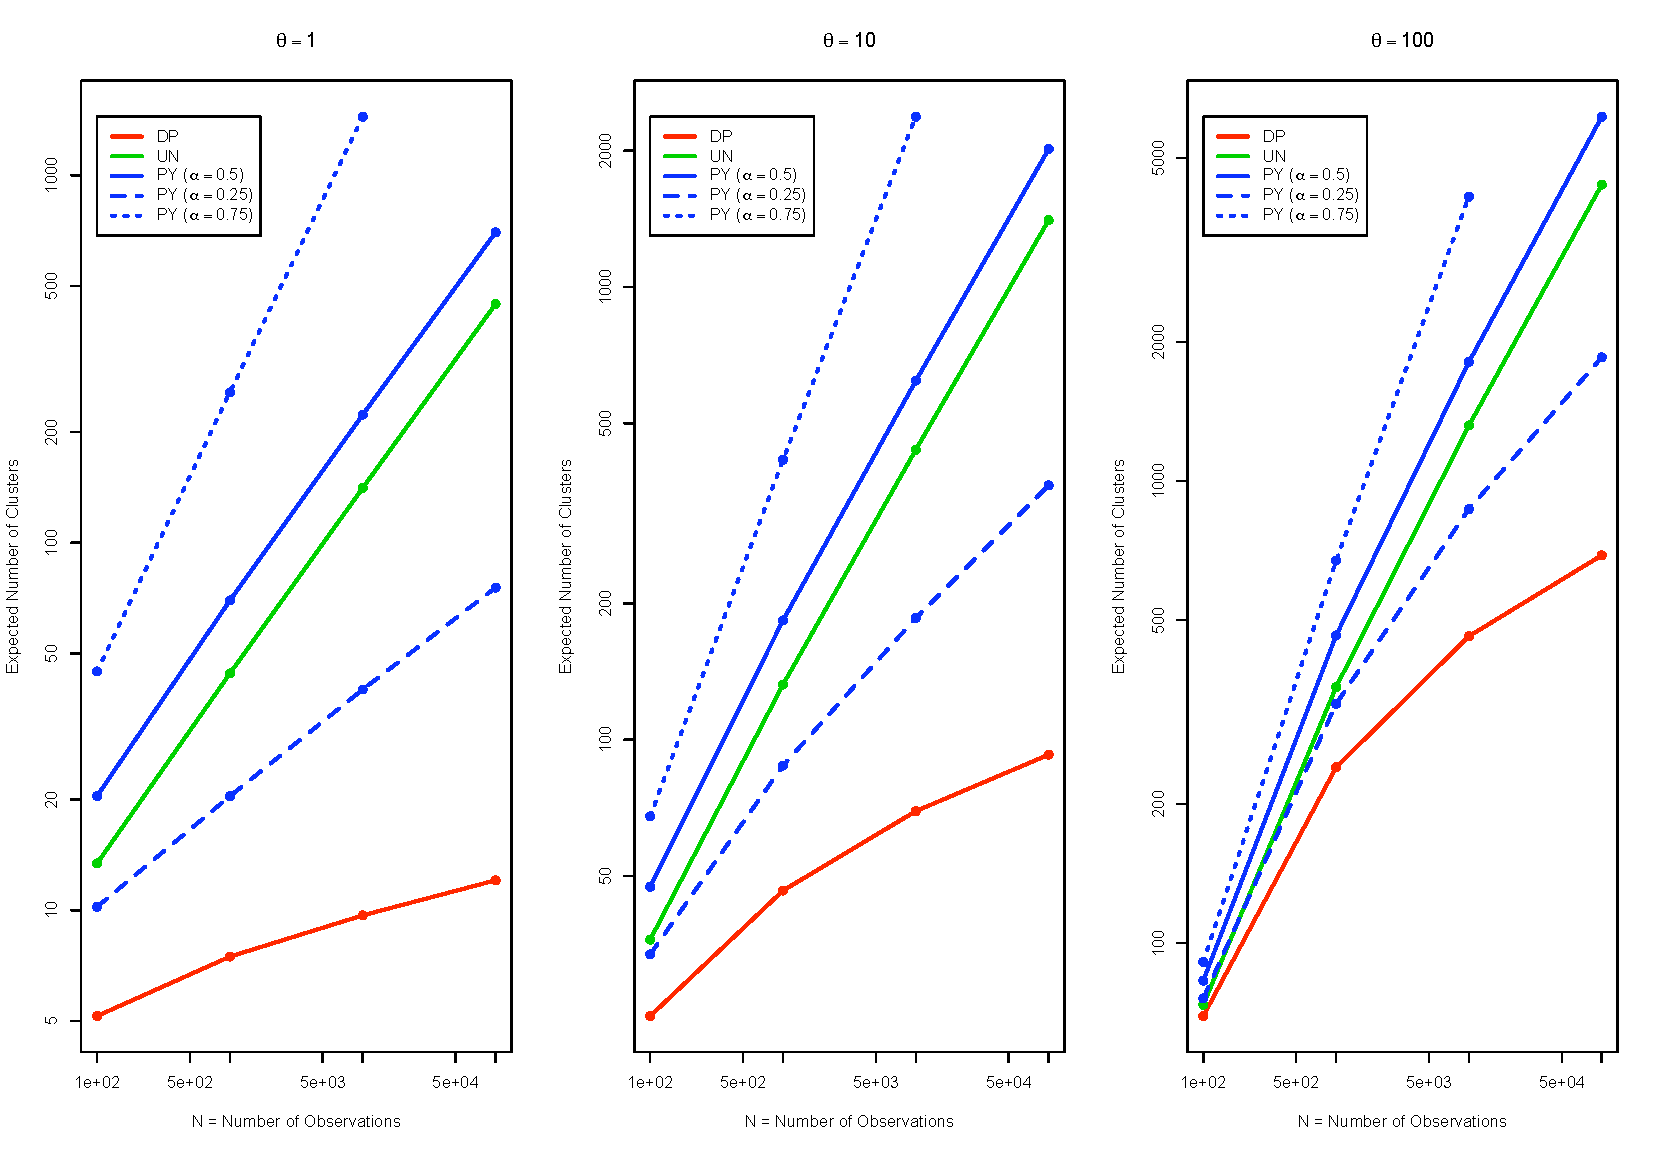
\includegraphics[width=5in,height=2in]{figures/fig_numberofclusters.pdf}
\caption{Expected number of clusters $\hat{K}_N$ as a function of
  sample size $N$ for different $\theta$ values.
\comment{ Axes are
on a log scale.}}\label{numberofclusters}
\vspace{-0.4cm}
\end{figure*}


\subsection{Comparison of Distribution of Cluster Sizes between
  Processes}

In this section, we examine the expected distribution of cluster sizes
under each process. For brevity, we focus on concentration parameter
$\theta = 10$ only, though the same trends are observed for other
values of $\theta$. Figure~\ref{simclustersizes} is a plot of
$\hat{H}_{M,N}$, the average number of clusters of size $M$, as a
function of $M$. For each process, $\hat{H}_{M,N}$ was calculated as
the average over the 1000 simulated independent partitions of
$H_{M,N}$ under that processes. Each red line indicates the asymptotic
relationship, i.e., (\ref{DPmom1}) for the Dirichlet process,
(\ref{PYmom4}) for the Pitman-Yor process and (\ref{UNmom4}) for the
uniform process.

The results in figure~\ref{simclustersizes} demonstrate that the
simulated distribution of the cluster sizes from the uniform process
is quite different to the simulated cluster size distributions for
either the Dirichlet process or the Pitman-Yor process.  It is also
interesting to observe the divergence from the asymptotic
relationships due to the finite sample sizes, especially in the case
of smaller $N$ (e.g., $N = 1000$).

\begin{figure*}[t]
\centering
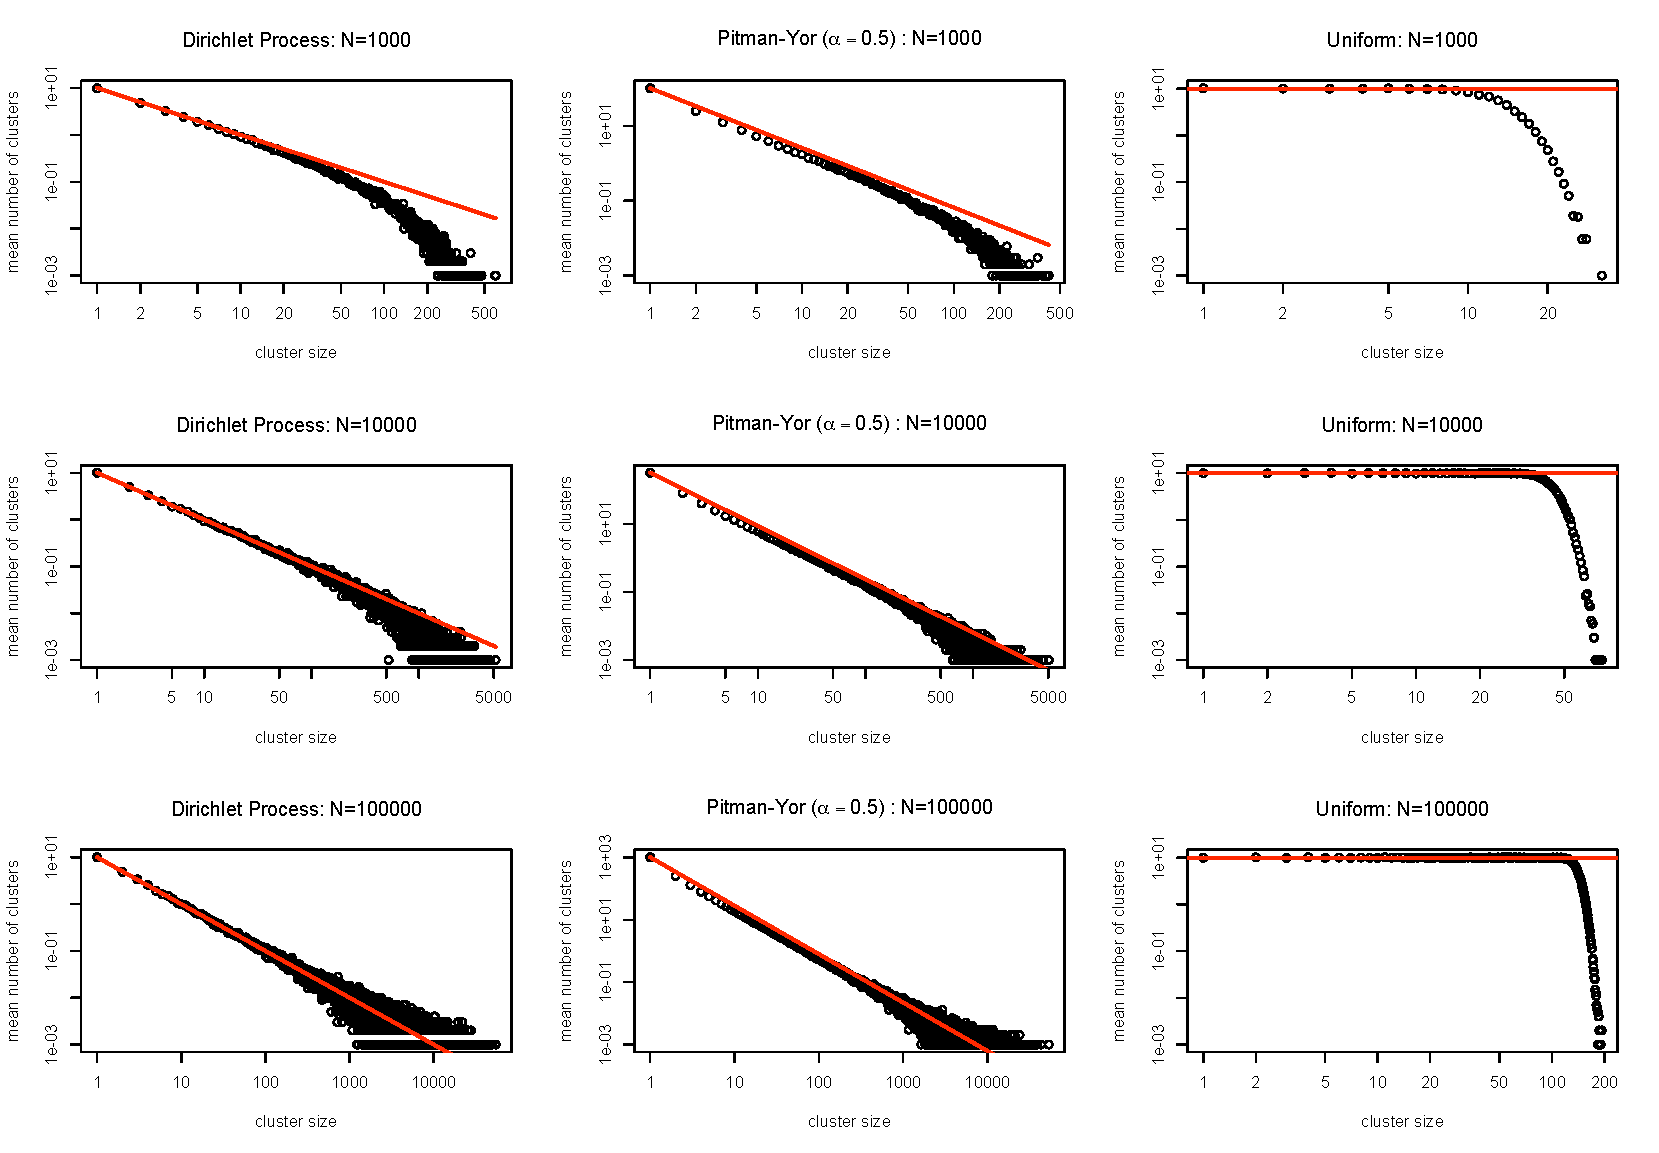
\includegraphics[width=5in,height=2.5in]{figures/fig_clustersizes.pdf}
\caption{Cluster sizes $H_{M,N}$ as a function of $M$ for different
  values of $N$ and the three different processes.  Data is plotted on a log-log
  scale and the red lines indicate the asymptotic
  relationships.}\label{simclustersizes}
\vspace{-0.4cm}
\end{figure*}

\section{Exchangeability}
\label{exchangeability}

As mentioned in section~\ref{priors}, the uniform process is not
exchangeable over observations. In this section, we explore this lack
of exchangeability by first examining, for real-world data, the extent
to which $P(\bc)$ is affected by permuting the observations. For any
particular ordering of observations $\bX = (X_1, \ldots, X_N)$, the
joint probability of the corresponding cluster assignments $\bc$ is
given by
\begin{equation}
P(\bc \g \textrm{ordering $1, \ldots, N$}) = \prod_{n=1}^N P(c_n \g \bc_{<n})
\end{equation}
where ``$\bc_{<n}$'' denotes the cluster assignments for observations $X_1,
\ldots, X_{n-1}$ and 
$P(c_n \g \bc_{<n})$ is given by (\ref{UNrule}). Clearly,
exhaustive evaluation of $P(\bc)$ for all possible orderings is not
possible for realistically-sized data sets. However, we can evaluate
the robustness of $P(\bc)$ to different orderings by first computing
the standard deviation of $\log{P(\bc)}$ for $L$ different partitions
$\bc$, inferred using the uniform process Gibbs sampling algorithm
described in the next section. This gives an estimate of the
variability of inferred partitions for a fixed ordering. For each
partition $\bc$ we can then compute the standard deviation of $\log
P(\bc)$ for different orderings of the observations, which gives an
estimate of the degree to which the ordering of observations affects
$P(\bc)$. Figure~\ref{orderingfig} shows the ``Between-Partition SD"
and ``Between-Ordering SD" for partitions of 1000 carbon
nanotechnology patent abstracts (see next section), obtained using
five Gibbs chains and 5000 orderings of the abstracts with different values of
$\theta$.  The variability between orderings is considerably smaller
than the variability between partitions, suggesting that uniform
process clustering results are not significantly sensitive to different
orderings. These results indicate that the lack of exchangeability
over observations exhibited by the uniform process is not a
significant issue for real-world clustering problems.

\begin{figure*}[t]
\vspace{-0.5cm}
\centering
\rotatebox{270}{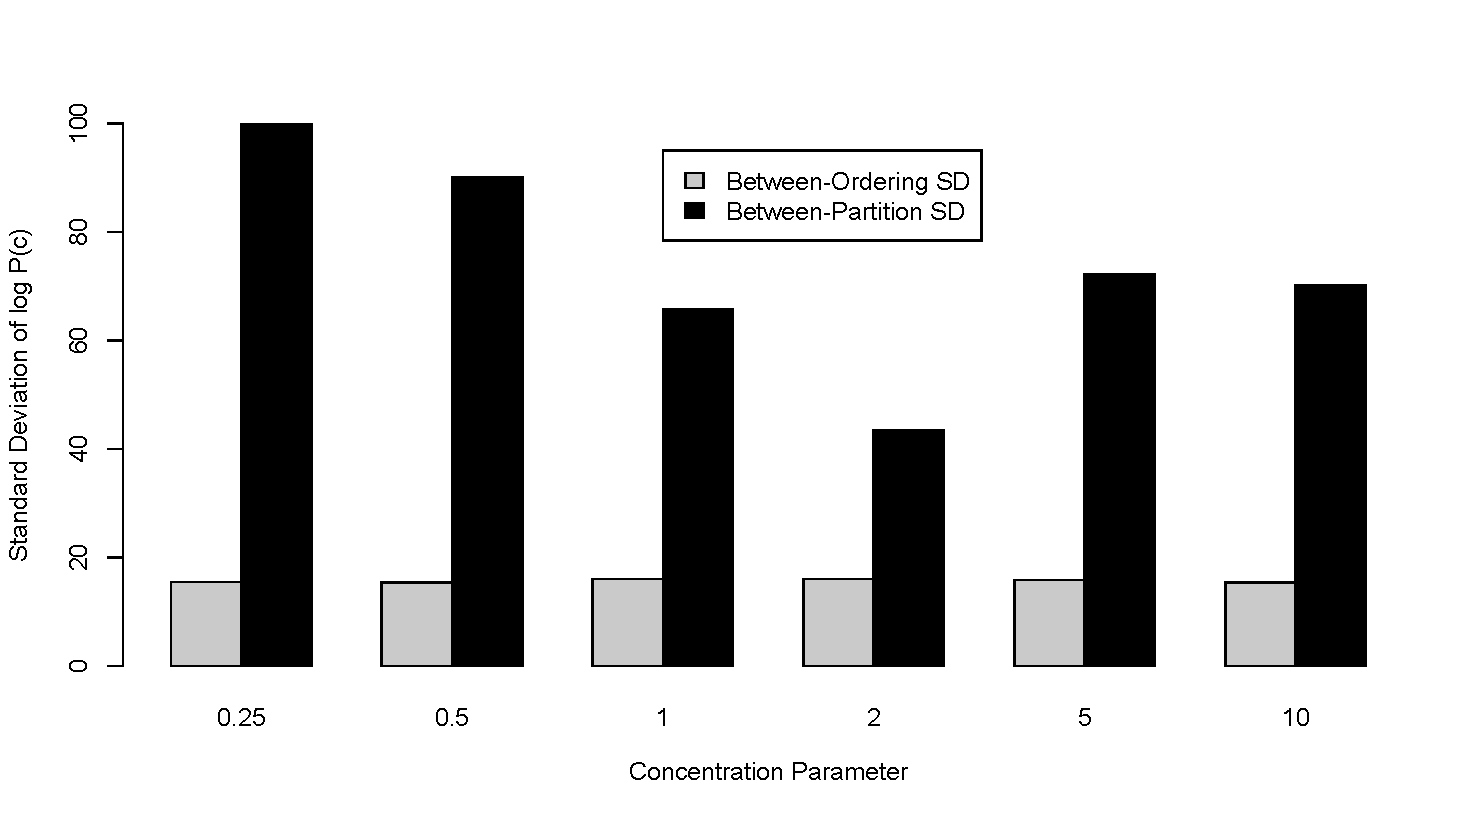
\includegraphics[width=4in,height=2.5in,angle=90]{figures/fig_results_sdcomp.pdf}}
\caption{Comparison of ``Between-Partition SD" and ``Between-Ordering
  SD" (averaged over different inferred partitions) for the uniform
  process with six values of concentration parameter
  $\theta$.}\label{orderingfig}
\vspace{-0.4cm}
\end{figure*}


\section{Application to Document Clustering}\label{application}

In this section, we compare the Dirichlet and uniform processes on the
task of clustering real-world documents---specifically the abstracts
from 1200 carbon nanotechnology patents.  Dirichlet processes have
been used as the basis of many document clustering models including
those of Zhang et al.~\cite{ZhaGhaYan05}, Zhu et
al.~\cite{ZhuGhaLaf05} and Wallach~\cite{Wal08}. In practice, however,
it is often the case for these tasks that there is no reason to
justify the \emph{a priori} ``rich-get-richer'' property exhibited by
the Dirichlet process.

We consider a nonparametric word-based mixture model where documents
are clustered into groups on the basis of word occurrences. The model
assumes the following generative process: the tokens $\bw_d$ that
comprise each document, indexed by $d$, are drawn from a
document-specific distribution over words $\bphi_d$, which is itself
drawn from a document-specific Dirichlet distribution with base
measure $\bn_d$ and concentration parameter $\beta$. The base measure
$\bn_d$ is distributed according to
\begin{equation*}
P(\bn_d \g G) = G(\bn_d)
\end{equation*}
where
\begin{equation*}
P(G \g \theta, G_0) = \textrm{DP}\,(G \g \theta, G_0) \textrm{ or }
\textrm{UP}\,(G \g \theta, G_0).
\end{equation*}
$G$ is is a random probability measure distributed according to either
a Dirichlet or uniform process with base measure $G_0$ and
concentration parameter $\theta$. Finally, $G_0$ is chosen to be a
hierarchical Dirichlet distribution: $G_0 = \textrm{Dir}\,(\bn_{c} \g
\beta_1 \bn)$, where $\bn \sim \textrm{Dir}\,(\bn \g \beta_0
\bu)$. (See supplementary materials for the complete graphical model.)
This model captures the fact that documents in different clusters will
likely use different vocabularies, while allowing the distribution
over words for each document to vary slightly from the word
distribution for the cluster to which that document belongs.

The key consequence of using either a Dirichlet or uniform process
prior is that the latent variables $\bn_d$ are partitioned into $C$
clusters where $C$ does not have to be pre-specified and fixed.  The
vector $\bc$ denotes the cluster assignments for each document: $c_d$
is the cluster assignment for document $d$.  Given a set of observed documents
$\mathcal{W} = \{\bw_d \}_{d=1}^D$, we can use Gibbs
sampling~\cite{geman84stochastic} to infer the latent cluster
assignments $\bc$.  Specifically, the cluster assignment $c_d$ for
document $d$ is resampled from
\begin{eqnarray}
p(c_d \g \bc_{\setminus d}, \bw, \theta) \, \propto \, p(c_d \g \bc_{\setminus d}, \theta) \, \cdot \, p(\bw_d \g c_d,
\bc_{\setminus d}, \mathcal{W}_{\setminus d}, \bbeta),\label{gibbssampling}
\end{eqnarray}
where $\bc_{\setminus d}$ and $\mathcal{W}_{\setminus d}$ denote the
sets of clusters and documents, respectively, excluding document $d$.
The vector $\bbeta = (\beta, \beta_1, \beta_0)$ represents the other
parameters in the model, which can be inferred using slice
sampling~\cite{neal03slice}, as described by Wallach~\cite{Wal08}. The
likelihood component of (\ref{gibbssampling}) is
\begin{eqnarray}
p(\bw_d \g c_d,
\bc_{\setminus d}, \mathcal{W}_{\setminus d}, \bbeta) \, = \, \prod_{n=1}^{N_d} \frac{N_{w_n|d}^{<d,n} + \beta\,
  \frac{N_{w_n|c_d}^{<d,n} + \beta_1\, \frac{N_{w_n}^{<d,n} + \beta_0\,
      \frac{1}{W}}{\sum_w N_w^{<d,n} + \beta_0}}{\sum_w N_{w|c_d}^{<d,n} +
    \beta_1}}{\sum_w N_{w|d}^{<d,n} + \beta},
\end{eqnarray}
where ``$< d,n$'' denotes a quantity including data from documents $1,
\ldots, d$ and positions $1, \ldots, n-1$ only for document
$d$. $N_{w|d}$ is the number of times word type $w$ occurs in document
$d$, $N_{w|c_d}$ is the number of times $w$ occurs in cluster $c_d$,
and $N_w$ is the number of times $w$ occurs in the entire corpus.

The conditional prior probability $P(c_d \g \bc_{\setminus d},
\theta)$ can be constructed using any of the predictive probabilities
in section~\ref{priors}. For the sake of brevity, we focus on
comparing the (commonly-used) Dirichlet process with the uniform
process. For the Dirichlet process, the conditional prior probability
is 
\begin{equation}
p(c_d \g \bc_{\setminus d}, \theta) \propto \begin{cases} N_{c_d} &
  c_d \textrm{ is an existing cluster}\\ \theta & c_d \textrm{ is a
    new cluster.} \end{cases}
\end{equation}
Since the uniform process lacks exchangeability over observations, we
condition upon an arbitrary ordering of the documents, e.g., $1,
\dots, D$. The conditional prior of $c_d$ given $\bc_{\setminus d}$ is
therefore
\begin{equation}
P(c_d \g \bc_{\setminus d}, \theta, \textrm{ ordering $1, \ldots, D$}) \propto P(c_d \g c_1,\ldots,c_{d-1}, \theta) \prod_{m=d+1}^{D} P(c_m \g c_1,\ldots,c_{m-1}, \theta),
\end{equation}
where $P(c_d \g c_1,\ldots,c_{d-1}, \theta)$ is given by the
predictive probability (\ref{UNrule}).  This expression propagates the
value of $c_d$ to the cluster assignments $c_{d+1}, \ldots, c_D$ of the
documents that follow document $d$ in the chosen ordering. With this
definition of the conditional prior, the Gibbs sampling algorithm is a
correct clustering procedure for $\mathcal{W}$, conditioned on the
arbitrarily imposed ordering of documents.  \comment{In the next
  section we investigate the extent to which the choice of imposed
  ordering affects $P(\bc)$.}

We compare the Dirichlet process and uniform process priors by using
the model (with each prior) to cluster the abstracts from 1200 carbon
nanotechnology patents. For each prior, we use Gibbs sampling and
slice sampling to infer cluster assignments $\bc^{\textrm{train}}$ and
$\bbeta$ for a subset $\mathcal{W}^{\textrm{train}}$ of 1000
``training'' abstracts. Since the results in
section~\ref{exchangeability} indicate that the variability between
partitions is greater than the variability between orderings, we use a
single ordering of $\mathcal{W}^{\textrm{train}}$ and perform five
runs of the Gibbs sampler. To provide insight into the role of
concentration parameter $\theta$, we do not allow $\theta$ to vary,
but instead compare results for several fixed $\theta$ values. We
evaluate predictive performance using a held-out set
$\mathcal{W}^{\textrm{test}}$ of 200 abstracts and computing the
probability of this held-out set given each run from trained model.
We compute $\log{P(\mathcal{W}^{\textrm{test}} \g
  \mathcal{D}^{\textrm{train}}, \theta, \bbeta)} =
\log{\sum_{\bc^{\textrm{test}}} P(\mathcal{W}^{\textrm{test}},
  \bc^{\textrm{test}} \g \mathcal{D}^{\textrm{train}}, \theta,
  \bbeta)}$, where $\mathcal{D}^{\textrm{train}} =
(\mathcal{W}^{\textrm{train}}, \bc^{\textrm{train}})$ and the sum over
held-out cluster assignments $\bc^{\textrm{test}}$ is approximated
using a novel variant of Wallach et al.'s ``left-to-right'' evaluation
algorithm~\cite{wallach09evaluation} (see supplementary materials). We
average this quantity over runs of the Gibbs sampler for
$\mathcal{W}^{\textrm{train}}$, runs of the evaluation algorithm and
twenty permutations of the held-out data.

The left-hand plot of figure~\ref{resultsfig} shows a comparison of
the Dirichlet process and the uniform process in terms of
$\log{P(\mathcal{W}^{\textrm{test}} \g \mathcal{D}^{\textrm{train}},
  \theta, \bbeta)}$. Regardless of the value of the concentration
parameter $\theta$, the model based on the uniform process leads to
systematically higher probabilities of the held-out data than the
model based on the Dirichlet process. Evidently the uniform process
provides a substantially better fit for the data in this application.
The right-hand plot of figure~\ref{resultsfig}, shows a comparison of
the Dirichlet and uniform processes in terms of the average number of
clusters in a representative partition obtained using the Gibbs
sampler.  We see that the uniform process leads to a greater number of
clusters than the Dirichlet process for each value of $\theta$.  This
is not a surprising result given the theoretical results for the {\it
  a priori} expected cluster sizes (section~\ref{asymptotics}) and the
fact that the choice of clustering prior is clearly influential on the
posterior distribution in this application.
\begin{figure*}[t]
\vspace{-0.25cm}
\centering
\rotatebox{270}{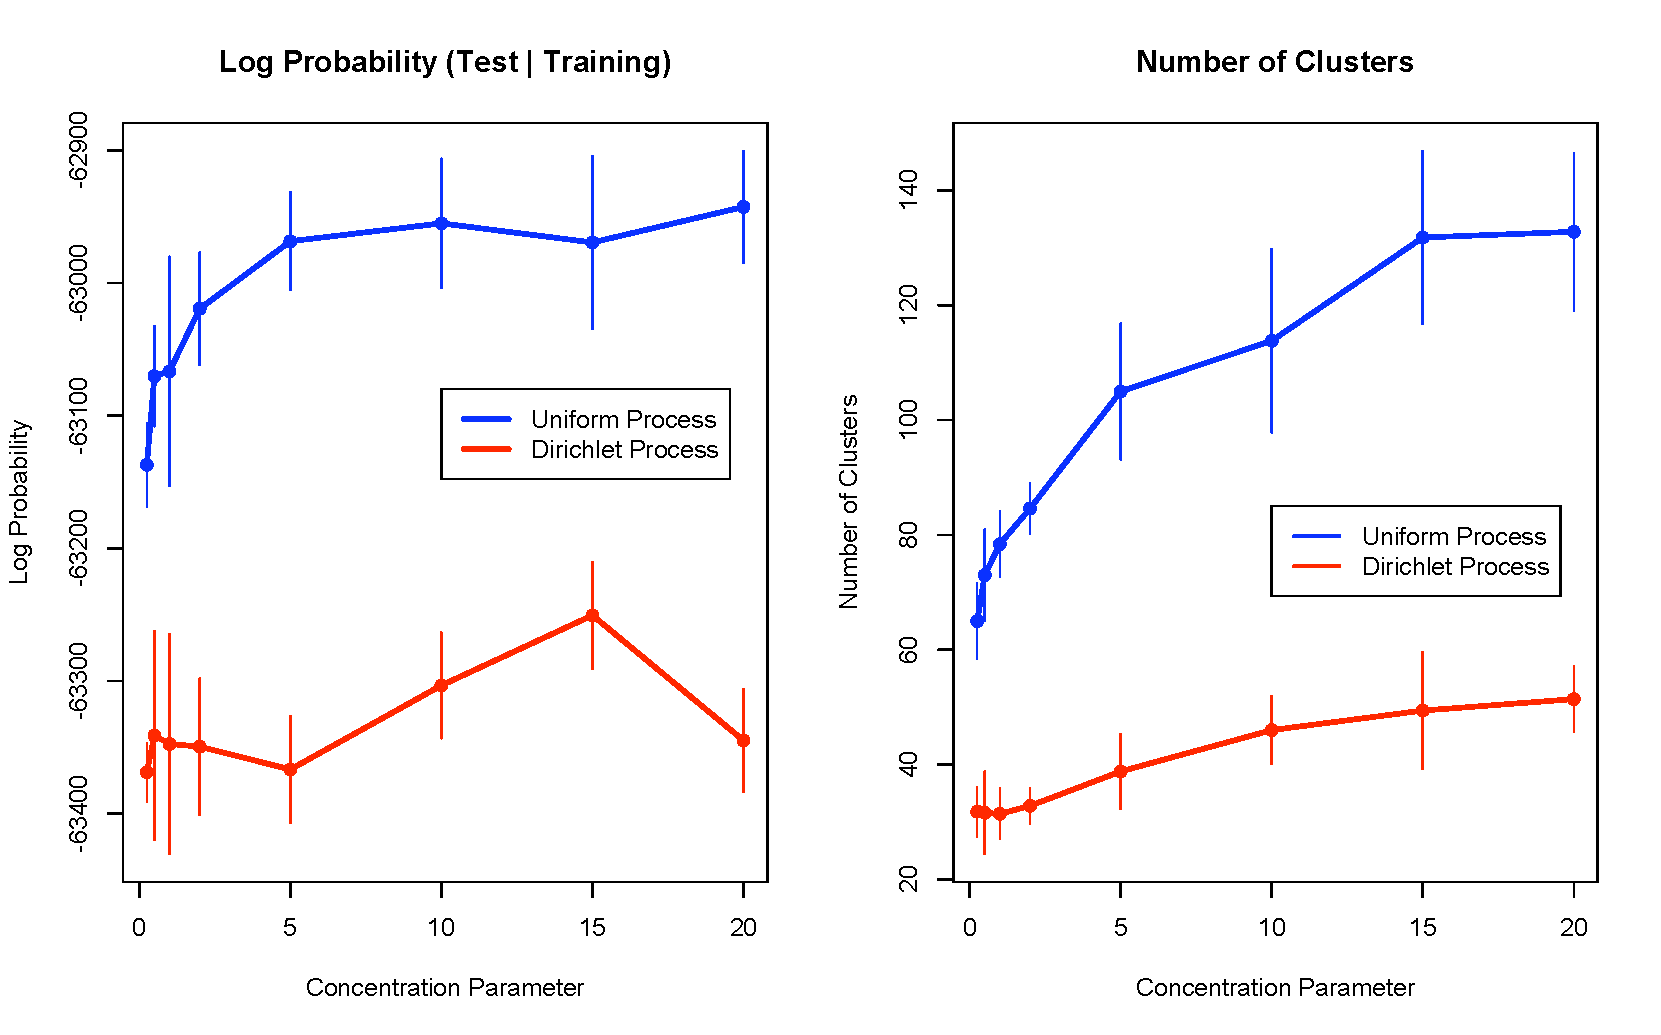
\includegraphics[width=5in,height=2.5in,angle=90]{figures/fig_results_combined.pdf}}
\caption{Comparison of Dirichlet and uniform process clustering models
  applied to carbon nanotechnology patent abstracts. Left: The average log
  probability of the held-out data given the trained model. The
  vertical lines indicate one standard deviation across runs of the
  Gibbs sampler for $\mathcal{W}^{\textrm{train}}$, runs of the
  evaluation algorithm and (for the uniform process) twenty
  permutations of the held-out data. Right: The average number of clusters
  in a representative partition from each trained model. The vertical
  lines indicate one standard deviation across runs of the Gibbs
  sampler for $\mathcal{W}^{\textrm{train}}$.}\label{resultsfig}
\vspace{-0.4cm}
\end{figure*}

%we are confident that the superior performance of the
%uniform process demonstrated in section~\ref{application} is robust to
%the arbitrary ordering imposed to address exchangeability.

\section{Discussion}\label{discussion}

The Dirichlet and Pitman-Yor processes both exhibit a
``rich-get-richer'' property that leads to partitions with a small
number of relatively large clusters. This property is seldom fully
acknowledged by practitioners when using either process as part of a
nonparametric Bayesian clustering model. In this paper, we have
examined the uniform process prior, which eliminates this
``rich-get-richer'' property. The uniform process prior has received
relatively little attention in the statistics and machine learning
literature to date, and its clustering characteristics have remained
largely unexplored. We have provided a comprehensive comparison of the
uniform process with the better-known Dirichlet and Pitman-Yor
processes and presented a new asymptotic result for the square-root
growth of the expected number of clusters under the uniform process.
We also conducted a simulation study for finite sample sizes that
demonstrates a substantial difference in the distribution of cluster
sizes between the uniform process and the Pitman-Yor and Dirichlet
processes. Previous work on the uniform process has ignored its lack
of exchangeability over observations. We present new results
demonstrating that although the uniform process is not invariant to
permutations of the observations, it is highly robust. Finally, we
compare the uniform and Dirichlet processes on a real-world document
clustering task, demonstrating superior predictive performance of the
uniform process over the Dirichlet process.

\comment{
\section*{Acknowledgment}
The authors thank Warren Ewens, Dylan Small and David Mimno for many
helpful discussions.
}

\newpage

\bibliographystyle{abbrv}
\bibliography{references}

\end{document}
